\documentclass{beamer}
\usetheme{Boadilla}

% Paquetes
%===================================================================================================

% % Paquete para incluir codigo
\usepackage{listings}

% Paquete para incluir imagenes
\usepackage{graphicx}
\graphicspath{ {./Imagenes/} }

% % Para la bibliografia
% % Sin esto, los enlaces de la bibliografia dan un error de compilacion
\usepackage{url}

% % Para enlaces clickables
\usepackage{hyperref}

% Metadatos del documento
%===================================================================================================
\title{
    {Metaheurísticas - Proyecto Final}\\
    {\emph{Battle Royale Metaheuristic}}\\
    {\emph{Cec17 Competition}}
}

\author{
    {Sergio Quijano Rey - 72103503k}\\
    {sergioquijano@correo.ugr.es} \\
    {4º Doble Grado Ingeniería Informática y Matemáticas}
}

\date{\today}

% Separacion entre parrafos
\setlength{\parskip}{1em}

% Contenido del documento
%===================================================================================================
\begin{document}

% Transparencia del titulo
\begin{frame}
    \titlepage
\end{frame}

% Transparencia con la tabla de contenidos
\begin{frame}
    \frametitle{Contenidos}
    \tableofcontents
\end{frame}

\section{Identificación del problema a resolver}

\begin{frame}
\frametitle{Problema a resolver}

El problema a resolver consiste en realizar una propuesta de metaheurística original para problemas de codificación real. A partir de esta propuesta, realizaremos una implementación de dicha metaheurística original, y trabajaremos la competición \emph{Cec17}.

\end{frame}

\subsection{Software de Daniel Molina}
\begin{frame}
\frametitle{Software de Daniel Molina}
    \begin{itemize}
        \item Para trabajar con la competición \emph{Cec17}
        \item Se encuentra en \url{https://github.com/dmolina/cec2017real}
    \end{itemize}
\end{frame}

\begin{frame}
El software contiene:

\begin{itemize}
    \item Librería escrita en \lstinline{C} que define las 31 funciones de \emph{fitness} que debemos optimizar, para las distintas dimensiones disponibles, así como otras funcionalidades
    \item Código \lstinline{python} para generar unas tablas \emph{Excel} que podemos usar en \href{tacolab.org}{tacolab.org} para comparar con otros algoritmos de referencia
    \item Wrapper para \lstinline{Python}, con el que podemos acceder a todas las funciones definidas en la ya mencionada librería dinámica
\end{itemize}
\end{frame}

\subsection{Casos de uso a estudiar}
\begin{frame}
\frametitle{Casos de uso a estudiar}

Por no tener que lidiar con tiempos de ejecución muy largos, los profesores de prácticas nos indican:

\begin{itemize}
    \item Debemos estudiar el comportamiento sobre 31 funciones distintas
    \item Debemos trabajar con dimensión 10 y 30
    \item Por cada función y dimensión, debemos lanzar 10 ejecuciones de la búsqueda
\end{itemize}
\end{frame}

\section{Nuestra metaheurística}

\subsection{Código de la metaheurística}
\begin{frame}
    \frametitle{Nuestro código}
    \begin{itemize}
        \item Nuestro código se encuentra alojado en un repositorio de \emph{Github}
        \item \url{https://github.com/SergioQuijanoRey/PracticaFinalMetaheuristicas}
    \end{itemize}
\end{frame}

\subsection{Inspiración de la metaheurística}

\begin{frame}
    \frametitle{Inspiración de la metaheurística}

    \begin{itemize}
        \item Basado en el género de videojuegos \emph{Battle Royale}
        \item Este género de videojuegos se inspira a su vez en la trilogía \emph{Los juegos del hambre}
    \end{itemize}

    \begin{figure}
        \centering
        
\includegraphics[width=0.5\textwidth]{portada}
    \end{figure}

\end{frame}

\subsection{Dinámicas del juego}
\begin{frame}
    \frametitle{Dinámicas del juego}
    Las dinámicas que introducen estos juegos son:

    \begin{itemize}
        \item 50 o 100 jugadores compitiendo
        \item Los jugadores aparecen en el mapa
        \item Fase inicial de recolección de recursos
        \item Fase final en la que el círculo se cierra
        \item Batallas entre dos jugadores
        \item Jugadores que reviven aleatoriamente
    \end{itemize}
\end{frame}

\begin{frame}
    \frametitle{50 o 100 jugadores compitiendo}

    \begin{itemize}
        \item Una gran cantidad de jugadores compiten por ser los últimos vivos en la partida
        \item Por tanto, nuestra metaheurística va a tener un carácter poblacional
    \end{itemize}
\end{frame}

\begin{frame}
    \frametitle{Los jugadores aparecen en el mapa}

    \begin{itemize}
        \item Modelamos esta primera fase como un fenómeno aleatorio
        \item Por tanto, partimos de una población con soluciones aleatorias
    \end{itemize}

    \begin{figure}
        \centering
        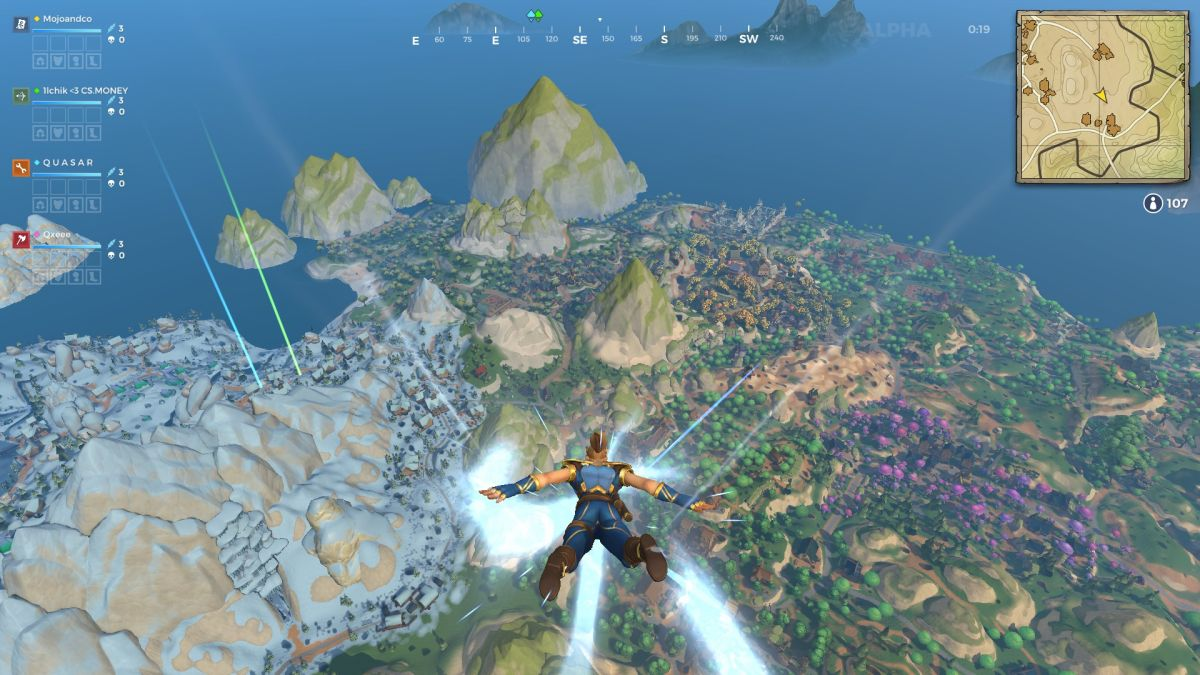
\includegraphics[width=0.5\textwidth]{jumping}
    \end{figure}
\end{frame}

\begin{frame}
    \frametitle{Fase inicial de recolección de recursos}

    \begin{itemize}
        \item Los jugadores aparecen en el mapa sin recursos
        \item En esta fase, buscan recursos por el mapa para ser más competitivos
        \item Esto se refleja en las búsquedas locales iniciales
    \end{itemize}

    \begin{figure}
        \centering
        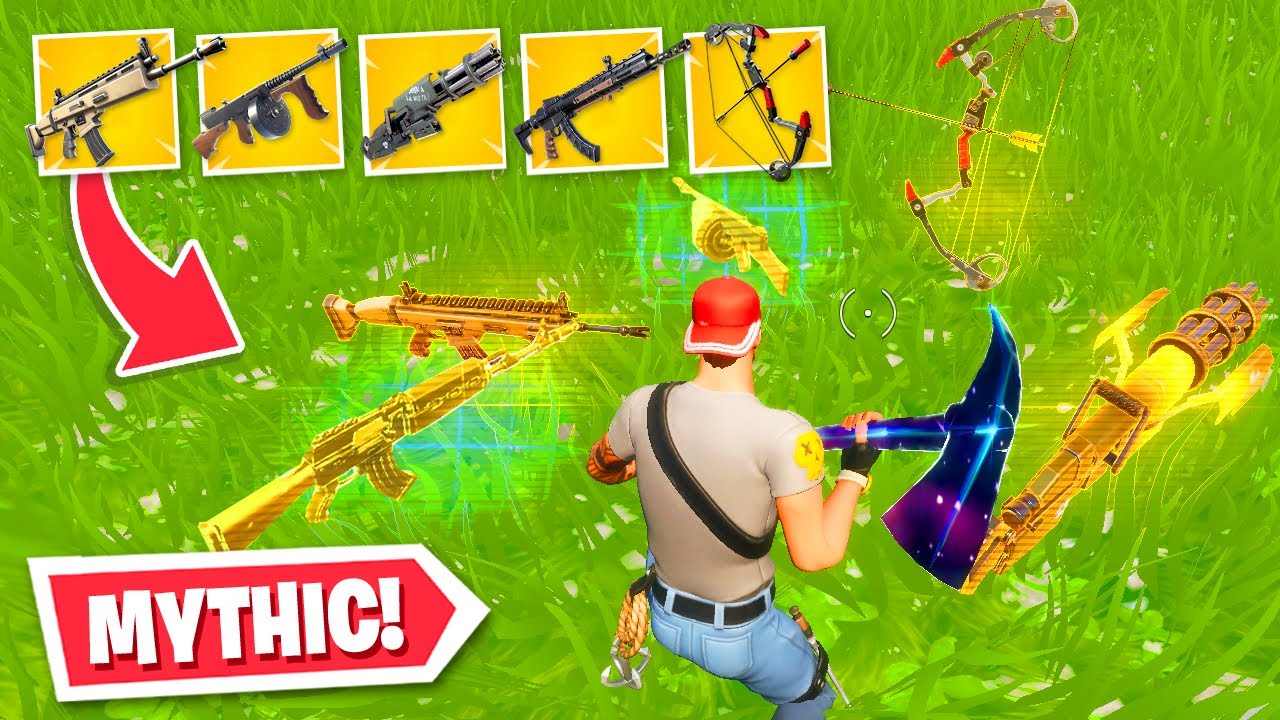
\includegraphics[width=0.5\textwidth]{resources}
    \end{figure}
\end{frame}

\begin{frame}
    \frametitle{Fase final en la que el círculo se cierra}

    \begin{itemize}
        \item A partir de cierto momento se cierra el mapa, muriendo los jugadores que queden fuera de la nueva zona
        \item Representamos esto haciendo un cierre no en el espacio, sino en el rango de \emph{fitness} de los jugadores
    \end{itemize}

    \begin{figure}
        \centering
        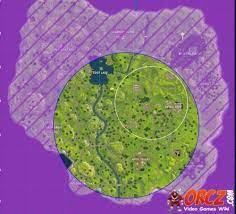
\includegraphics[width=0.5\textwidth]{circle}
    \end{figure}
\end{frame}

\begin{frame}
    \begin{figure}
        \centering
        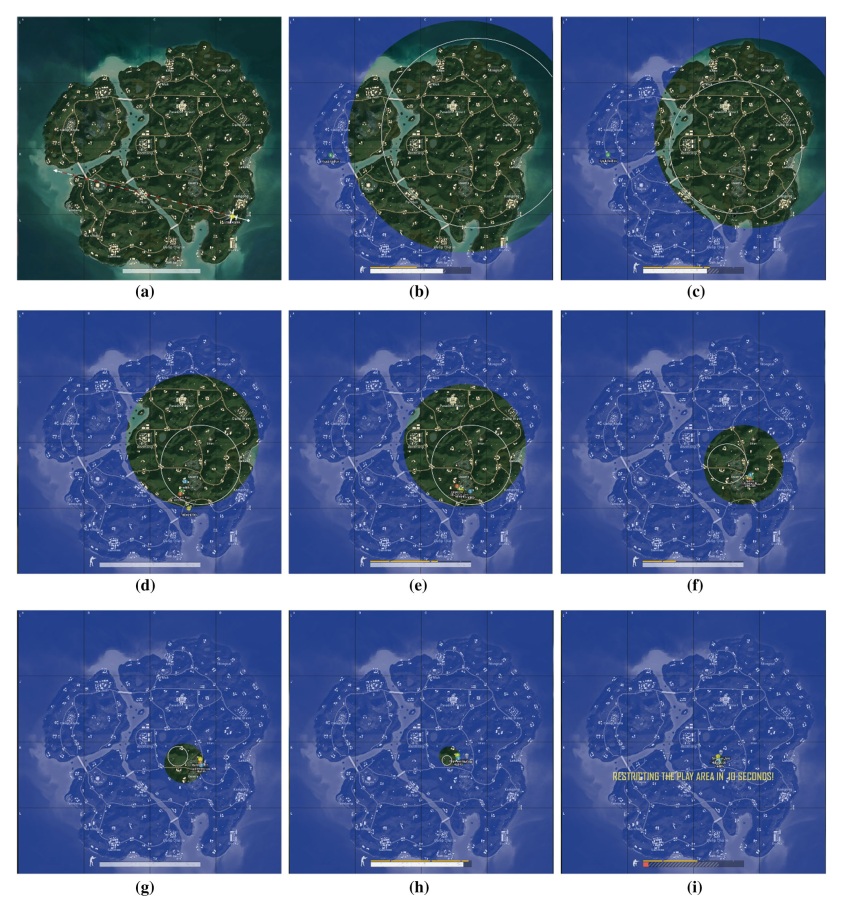
\includegraphics[width=0.6\textwidth]{cierre_circulo}
    \end{figure}
\end{frame}

\begin{frame}
    \frametitle{Batallas entre dos jugadores}

    \begin{itemize}
        \item Los jugadores cuando se cruzan pelean entre sí
        \item Cuando dos jugadores están cerca (en el sentido de la distancia Manhattan) pelean entre sí
        \item El mejor equipado (mejor \emph{fitness}) tiene más probabilidades de morir
    \end{itemize}

    \begin{figure}
        \centering
        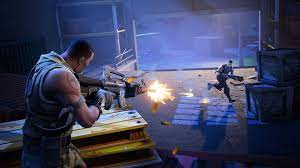
\includegraphics[width=0.6\textwidth]{fight}
    \end{figure}

\end{frame}

\begin{frame}
    \frametitle{Jugadores que reviven aleatoriamente}

    \begin{itemize}
        \item Cuando los jugadores mueren, tienen una pequeña probabilidad de resucitar \footnotemark
        \item Cuando resucitan, pierden todos los recursos almacenados y aparecen en una posición aleatoria
        \item Tienen un periodo de gracia en el que tienen que recolectar recursos para ser competitivos y entrar dentro del círculo
    \end{itemize}

    Esto se ve reflejado de la forma:

    \begin{itemize}
        \item Cuando un jugador revive, se le asigna una posición (solución) aleatoria
        \item Tras revivir, tiene una búsqueda local para que recolecte recursos y entre al círculo si puede en su tiempo de gracia
    \end{itemize}

    \footnotetext[1]{Esto no es común en los videojuegos de este género. Nos tomamos esta licencia para no perder variedad en la población, manteniendo una narrativa coherente}
\end{frame}

\subsection{Decisiones basadas en la ingeniería}

\begin{frame}
    \frametitle{Decisiones basadas en la ingeniería}

    Introducimos algunas variaciones basadas en decisiones de ingeniería

    \begin{itemize}
        \item Uso de la distancia Manhattan en vez de la distancia euclídea, pues es más rápida de computar
        \item Mecánica del cierre del círculo basada en el fitness de los jugadores en vez del restringir zonas del espacio de búsqueda
        \item Tras hacer \emph{parameter tuning}, la probabilidad de revivir no es baja, si no del 50\%
    \end{itemize}
\end{frame}

\end{document}
